\section{Detection of quadrature-squeezed vacuum states}\label{sec:vacuum-states-detection}
Suppose that a light field is sent onto a $50:50$ beam splitter, while a second strong field, called the \textbf{local oscillator} (LO), enters the other input port. The LO has a large amplitude but the same optical frequency as the signal field. The two output beams are detected by two photodetectors, and the resulting photocurrents are subtracted by a differential electronics stage. This configuration is called \textbf{balanced homodyne detection}. 
\begin{figure}[H]
    \centering
    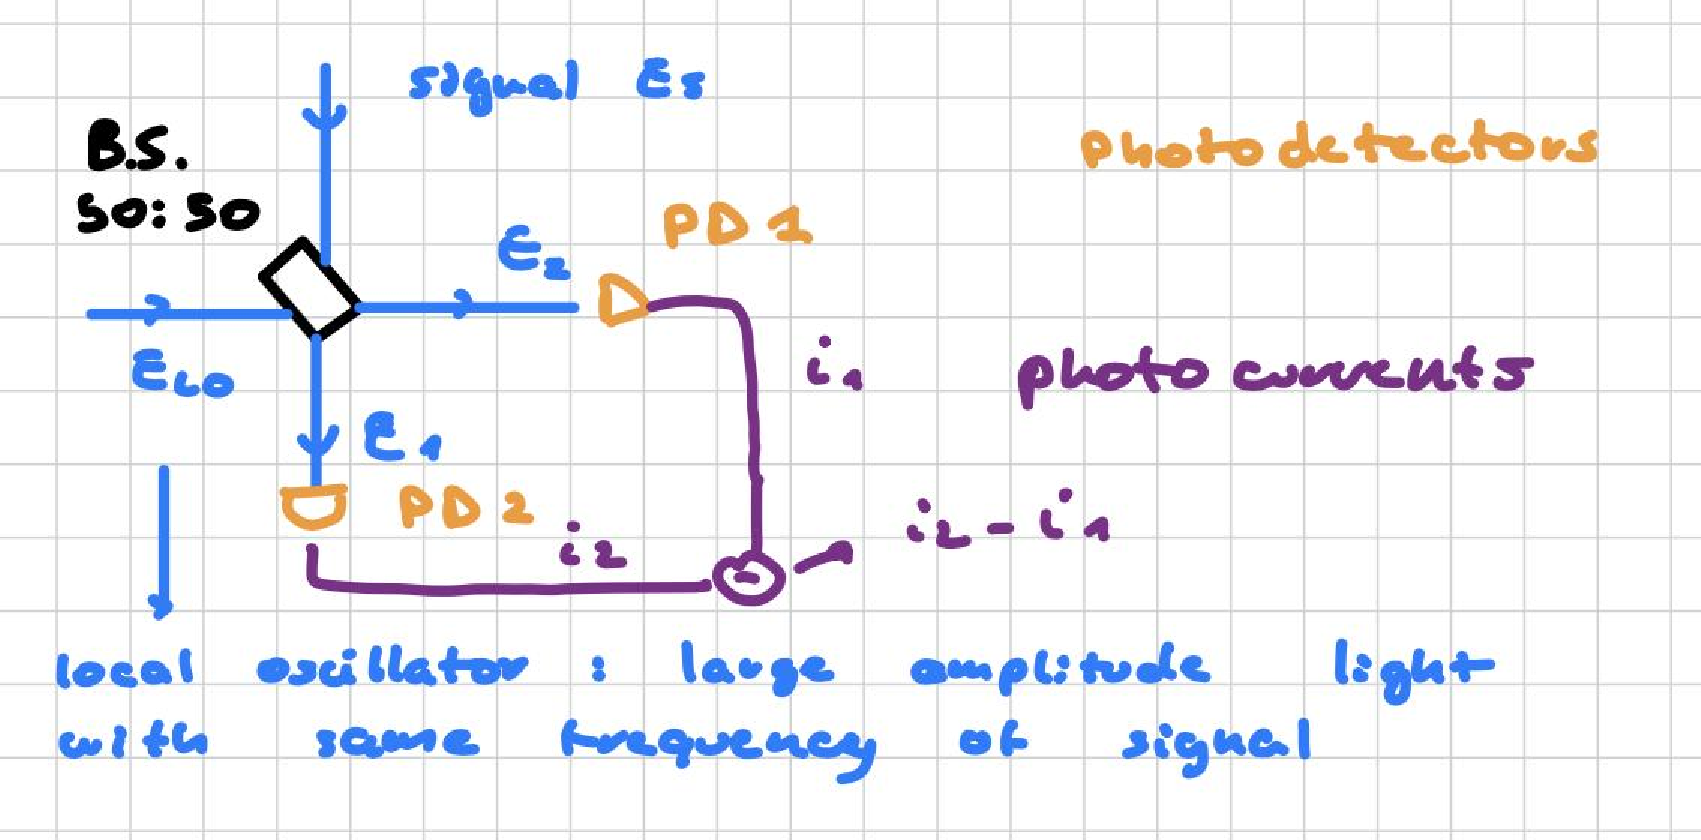
\includegraphics[width=0.6\linewidth]{images_in_pdf/14-/Grafico_79.pdf}
\end{figure}

We can distinguish two different situations:
\begin{enumerate}
    \item \textbf{No input at the signal port:} the local oscillator is equally split between the two detectors, so classically one expects
    \[
    i_2-i_1=0.
    \]
    However, because photons arrive randomly, each photodetector sees independent Poissonian fluctuations. Subtracting the two photocurrents removes the average signal, but it does not remove the quantum fluctuations, so the output still contains shot noise. For an ideal setup, the balanced detector has the same shot-noise level as a single detector measuring the same total optical power.
    \item \textbf{A signal field $E_s$ is present:}
    \[
    E_1=\frac{1}{\sqrt{2}}\left(E_{LO}e^{i\theta_{LO}}+E_s\right),
    \qquad
    E_2=\frac{1}{\sqrt{2}}\left(E_{LO}e^{i\theta_{LO}}-E_s\right).
    \]
    The local oscillator is a strong field and can therefore be treated classically, whereas the signal field is weak and must be treated quantum mechanically. We can decompose it into quadrature components:
    \[
    E_s=E_s^{x_1}+iE_s^{x_2}.
    \]
    Then the two output fields can be written as
    \[
    E_1=\frac{1}{\sqrt{2}}\Big[(E_{LO}\cos\theta_{LO}+E_s^{x_1})
    +i(E_{LO}\sin\theta_{LO}+E_s^{x_2})\Big],
    \]
    \[
    E_2=\frac{1}{\sqrt{2}}\Big[(E_{LO}\cos\theta_{LO}-E_s^{x_1})
    +i(E_{LO}\sin\theta_{LO}-E_s^{x_2})\Big].
    \]
    Since the photocurrent is proportional to $|E|^2$, the differential output is
    \[
    i_2-i_1 \propto E_1E_1^*-E_2E_2^*
    \propto E_{LO}\Big[\cos(\theta_{LO})\,E_s^{x_1}
    +\sin(\theta_{LO})\,E_s^{x_2}\Big].
    \]
    Therefore:
    \begin{itemize}
        \item if $\theta_{LO}=0,\pi,2\pi,\dots$, the output is proportional to the amplitude quadrature $E_s^{x_1}$;
        \item if $\theta_{LO}=\frac{\pi}{2},\frac{3\pi}{2},\dots$, the output is proportional to the phase quadrature $E_s^{x_2}$.
    \end{itemize}
    In this way, \textbf{the balanced homodyne detector measures the signal quadrature that is in phase with the local oscillator.}
\end{enumerate}
Let us reconsider the case with no signal at the input port. In that case, vacuum modes enter the signal port and the output is proportional to
\[
i_2-i_1 \propto E_{LO}\,E_{\mathrm{vac}}.
\]
In the absence of a signal, the balanced homodyne detector measures the vacuum fluctuations, which set the shot-noise level. In this wiew the detector can be viewed as homodyning the local oscillator with the vacuum field. \\\\
For a squeezed vacuum state instead, one quadrature has reduced noise below this limit, while the orthogonal quadrature has increased noise. This reduction below shot noise cannot be explained classically. But \textbf{how can we genrate these states?}\\\\
Quadrature-squeezed states can be generated by nonlinear optics.\\\\
Suppose that a nonlinear crystal is pumped by an intense laser beam with frequency
\[
\omega_p=2\omega,
\]
while a weak seed field has frequency
\[
\omega_s=\omega.
\]
This is the \textbf{degenerate parametric amplifier} configuration:
\begin{figure}[H]
    \centering
    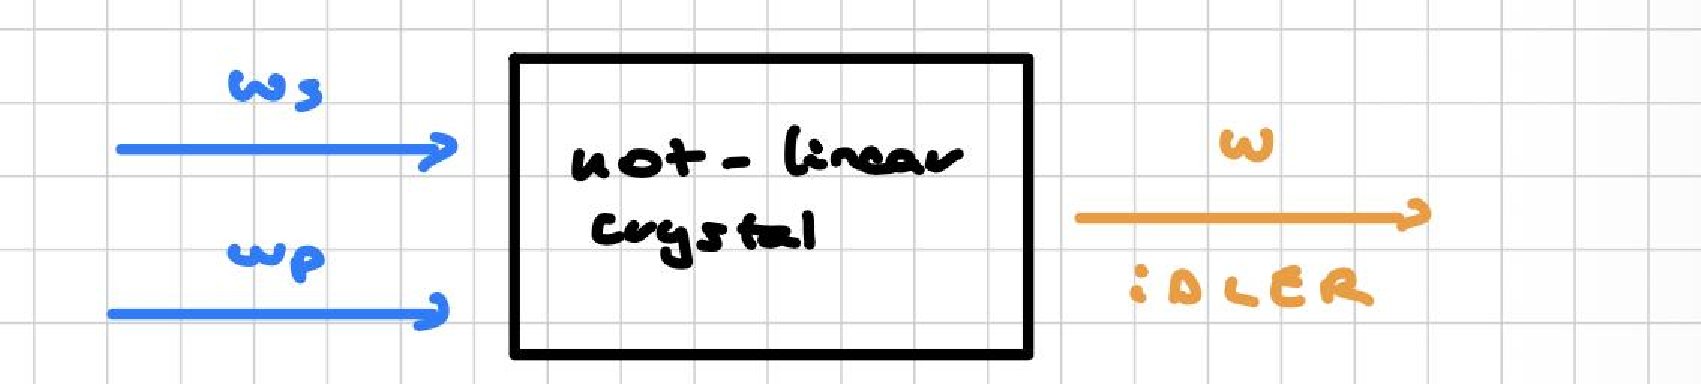
\includegraphics[width=0.6\linewidth]{images_in_pdf/14-/Grafico_80.pdf}
\end{figure}

In the degenerate case, the signal and idler fields have the same frequency:
\[
\omega_i=\omega_p-\omega_s=\omega.
\]
The nonlinear crystal mixes the pump and the signal through a $\chi^{(2)}$ interaction, so that the amplification of the field depends on the relative phase between the input signal and the pump. In the degenerate case, this phase-sensitive process can either amplify or deamplify a given field quadrature. If no signal is injected, the crystal acts on the vacuum field and converts vacuum fluctuations into a \textbf{squeezed vacuum} state.\\\\
In the absence of a seed, the only input at the signal port is the vacuum field, whose average amplitude is zero but whose fluctuations are not:
\[
E_{\mathrm{vac}} \sim \sqrt{\frac{\hbar\omega}{2\epsilon_0 V}}.
\]
\begin{figure}[H]
    \centering
    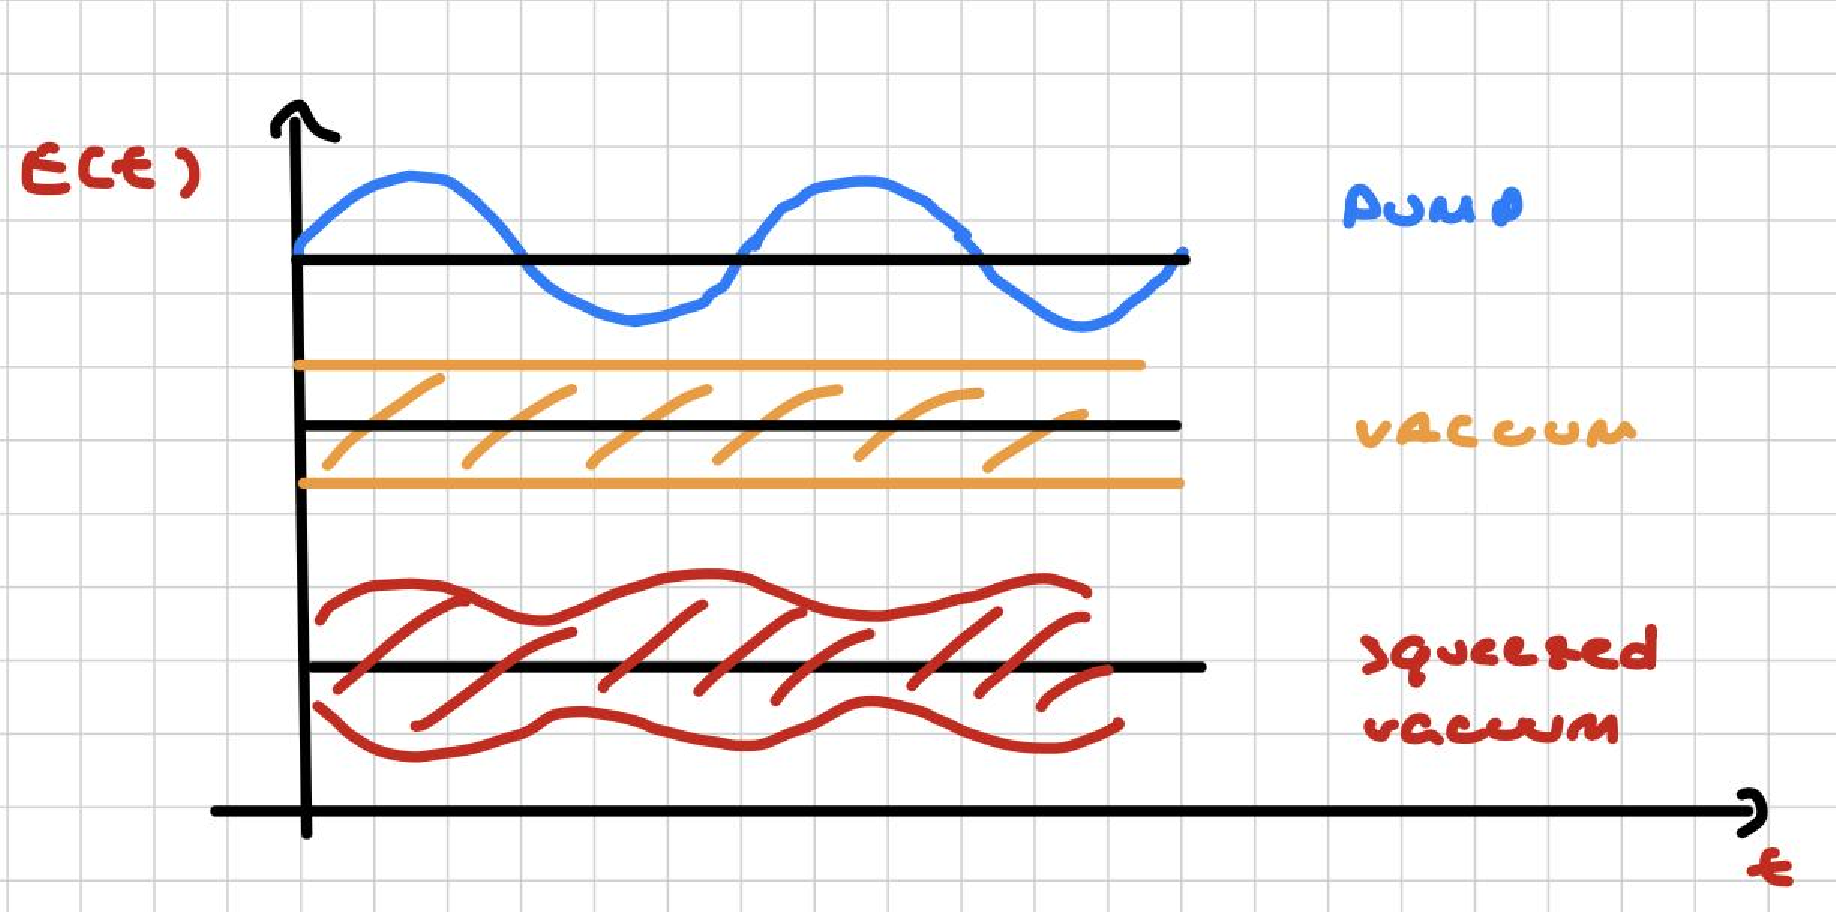
\includegraphics[width=0.6\linewidth]{images_in_pdf/14-/Grafico_81.pdf}
\end{figure}

\textbf{By changing the phase we can modulate the squeeze vacuum states and beat the shot noise:} Changing of phase correspond to select different field quadratures in the balanced homodyne detector. As result, one can observe either reduced noise below the shot-noise limit in the squeezed quadrature or increased noise above it in the conjugate quadrature $\implies$ the quantum noise is redistributed between two complementary quadratures. \\\\
This is the basic principle of squeezed-light metrology and is crucial in ultra-sensitive experiments, such as gravitational-wave detection, where reducing quantum noise is essential.